% !TeX root = ../main.tex
% Chapter 4
\chapter{Implementation Methodology and Step-by-Step Engineering Iterations}
\label{Chapter4}
\lhead{Chapter 4. \emph{Engineering Iterations}}

\section{Iterative Engineering Methodology}
Deploying zero-shot deep generative speech architectures to resource-constrained embedded systems requires addressing disparities between high-level machine learning frameworks (PyTorch, TorchScript) and physical edge execution environments (ARM NEON, Android NDK, Flutter runtime). These differences emerge across numerical precision, memory allocation, and linguistic tokenization boundaries.

To document the development of this project with academic rigor and experimental reproducibility, this chapter details the ten engineering iterations completed during this phase. Each iteration outlines:
\begin{enumerate}[label=(\roman*)]
    \item The operational objective and architectural hypotheses;
    \item The technical implementation and system modifications;
    \item The defects, runtime anomalies, or hardware bottlenecks encountered; and
    \item The algorithmic and systems-level resolutions applied.
\end{enumerate}

\section{Iteration 1: Mobile Feasibility Proof of Concept (ZipVoice-Distill via Sherpa-ONNX)}
\subsection{Objective: Testing Edge Flow-Matching Feasibility}
Before committing development resources to adapting a 335M parameter multilingual diffusion model for Indian languages, we first formulated an empirical proof of concept (PoC) to address a fundamental question: \textit{Can non-autoregressive continuous flow-matching speech synthesis execute zero-shot speaker adaptation directly on client mobile hardware within practical latency and memory budgets?}

To answer this question rapidly, we selected ZipVoice-Distill, an efficient, pre-quantized 123M parameter non-autoregressive Zipformer architecture. ZipVoice was selected as our PoC vehicle specifically because it was a mature, readily available flow-matching model with turnkey C++ mobile runtime support via \texttt{sherpa-onnx}~\cite{sherpaonnx2023}, providing pre-tested cross-platform Flutter/Android bindings.

\subsection{Implementation Details}
We developed the standalone evaluation script \texttt{english\_tts.py} (and legacy \texttt{zipvoice-tts.py}) utilizing the Python C++ bindings of \texttt{sherpa-onnx}. The PoC model architecture incorporated:
\begin{itemize}
    \item An INT8-quantized ZipVoice encoder (\texttt{encoder.int8.onnx}, ~5.5\,MB);
    \item An INT8-quantized Zipformer flow-matching decoder (\texttt{decoder.int8.onnx}, ~124\,MB);
    \item An espeak-ng Grapheme-to-Phoneme lexicon mapping English orthography to phonetic tokens; and
    \item A 24\,kHz Vocos vocoder graph (\texttt{vocos\_24khz.onnx}, ~54\,MB).
\end{itemize}

\subsection{Findings and Milestones}
Executing on a multi-core desktop CPU, the 4-step flow-matching engine cloned reference voices in approximately 1.8 to 2.4 seconds, achieving $\text{RTF} \approx 0.35$ for a 6-second utterance. This initial milestone confirmed that 4-step distilled continuous flow matching successfully avoids the multi-minute latency bottlenecks associated with classical score-based diffusion models.

\section{Iteration 2: Flutter Mobile PoC Prototype (\texorpdfstring{\texttt{voice\_clone\_proto}}{voice\_clone\_proto})}
\subsection{Objective and UI Architecture}
Following desktop validation, Iteration~2 migrated the PoC pipeline into a cross-platform Android mobile application named \texttt{voice\_clone\_proto}. The application was purposefully engineered as a teacher-facing classroom audio generator and an assistive learning tool for visually impaired students.

\subsection{System Implementation}
The application was built in Flutter using Material 3 design tokens, incorporating high-contrast layouts and Android TalkBack accessibility semantics to assist visually impaired learners. The user interface was structured into a guided 4-step workflow designed for rapid classroom lesson preparation:
\begin{enumerate}
    \item \textbf{Step 1: Reference Script Selection}: The teacher selects a phonetically balanced prompt phrase (such as \textit{``The quick brown fox jumps over the lazy dog''} or regional language equivalents) or enters custom text.
    \item \textbf{Step 2: Reference Audio Acquisition}: The teacher's voice is captured via live microphone recording (3 to 5 seconds) using the \texttt{record} package or imported from local storage via \texttt{file\_picker}.
    \item \textbf{Step 3: Target Text Entry}: The teacher enters textbook passages, conceptual explanations, or student quiz items categorized by duration presets (Short, Medium, Long).
    \item \textbf{Step 4: Generation and Waveform Playback}: Synthesizes the educational audio in the teacher's cloned voice and renders an interactive waveform visualization widget with tactile playback controls.
\end{enumerate}

\subsection{Concurrency and Background Isolate Decoupling}
Executing neural network inference on the main UI thread causes frame drops and triggers Android Application Not Responding (ANR) warnings. To maintain interface responsiveness, the Sherpa-ONNX C++ runtime was decoupled into a background \textbf{Dart Isolate} via \texttt{Isolate.run()}.

To handle arbitrary classroom recordings (such as AAC \texttt{.m4a} files captured on mobile handsets), we integrated an audio transcoding library based on FFmpeg to convert recordings into 16-bit 24\,kHz mono PCM WAV prior to inference.

\section{Iteration 3: Multi-Device Benchmarking of the PoC and Empirical Inferences}
\subsection{Benchmarking Methodology}
To evaluate hardware performance across silicon tiers, we deployed the \texttt{voice\_clone\_proto} PoC application across physical Android devices representing different performance brackets:
\begin{enumerate}
    \item \textbf{Flagship Tier}: Samsung Galaxy S23 (Qualcomm Snapdragon 8 Gen 2, 8\,GB RAM, dedicated NPU).
    \item \textbf{Upper Mid-Range Tier}: Samsung Galaxy Tab S9 FE+ (Samsung Exynos 1380, 8\,GB RAM, dedicated NPU).
    \item \textbf{Mid-Range Tier}: Samsung Galaxy M53 5G (MediaTek Dimensity 900, 8\,GB RAM, dedicated NPU).
    \item \textbf{Target Budget Baseline (Government School Hardware)}: Lenovo Tab K10 (MediaTek Helio P22T, 4\,GB RAM, CPU-only execution). This device serves as our primary engineering target because it represents the benchmark specification of subsidized tablets procured and distributed in bulk by Indian state education departments for rural classrooms and special education facilities.
\end{enumerate}

To measure exact physical memory consumption, the Flutter background isolate was instrumented to poll \texttt{/proc/self/status} directly from the Linux kernel virtual filesystem upon completion of each utterance:
\begin{lstlisting}[language=Java,caption={Dart In-Kernel Memory Profiling Hook via /proc/self/status}]
int rssMB = 0;
final file = File('/proc/self/status');
if (file.existsSync()) {
  for (final line in file.readAsLinesSync()) {
    if (line.startsWith('VmRSS:')) {
      final parts = line.split(RegExp(r'\s+'));
      if (parts.length >= 2) {
        rssMB = (int.tryParse(parts[1]) ?? 0) ~/ 1024;
        break;
      }
    }
  }
}
\end{lstlisting}

\subsection{Empirical Hardware Measurements}
Physical hardware benchmarking was conducted to measure computational throughput and memory behavior across physical Android silicon tiers. For the flagship, upper mid-range, and mid-range devices, previously collected benchmarks are reported using observed Real-Time Factors (\acrshort{rtf}) and reported resident memory readings (without continuous high-water-mark tracking).

For our primary hardware target, the \textbf{Lenovo Tab K10} (MediaTek Helio P22T, 4\,GB RAM, CPU-only execution), newly obtained experimental measurements evaluate nine independent synthesis trials across three standardized utterance-length tiers (Short, Medium, Long; three trials per tier). In each trial, Real-Time Factor is calculated from total execution latency, and post-utterance resident memory (\texttt{VmRSS}) is sampled directly from the Linux kernel virtual filesystem (\texttt{/proc/self/status}) upon completion of audio generation. Crucially, these measurements represent post-utterance resident memory rather than continuous peak RSS, and no \textit{LowMemoryKiller} terminations occurred across any of the nine trials.

Table~\ref{tab:empirical_benchmarks_detailed} summarizes throughput and memory behavior across device tiers, presenting arithmetic category means for the Lenovo Tab K10 alongside observed benchmark readings for other tiers. Table~\ref{tab:lenovo_raw_trials} records all nine individual experimental observations on the Lenovo Tab K10.

\begin{table}[htbp]
\centering
\caption[Empirical On-Device Benchmarks Across Physical Android Devices]{Empirical On-Device Benchmarks Across Physical Android Devices}
\label{tab:empirical_benchmarks_detailed}
\resizebox{\textwidth}{!}{%
\begin{tabular}{llccccc}
\toprule
\textbf{Device Model} & \textbf{Processor (SoC)} & \textbf{RAM} & \textbf{Utterance Tier} & \textbf{Throughput (RTF)} & \textbf{Resident Memory} & \textbf{Status / Trials} \\
\midrule
Samsung Galaxy S23 & Snapdragon 8 Gen 2 & 8\,GB & Short (~5w) & 3.826 (Observed\textsuperscript{*}) & 1,033\,MB (Reported RSS\textsuperscript{*}) & PASS (Observed) \\
Samsung Galaxy S23 & Snapdragon 8 Gen 2 & 8\,GB & Med (~25w) & 1.520 (Observed\textsuperscript{*}) & 1,287\,MB (Reported RSS\textsuperscript{*}) & PASS (Observed) \\
Samsung Galaxy S23 & Snapdragon 8 Gen 2 & 8\,GB & Long (~65w) & \textbf{1.288} (Observed\textsuperscript{*}) & \textbf{1,562\,MB} (Reported RSS\textsuperscript{*}) & PASS (Observed) \\
\midrule
Galaxy Tab S9 FE+ & Exynos 1380 & 8\,GB & Short (~5w) & 9.279 (Observed\textsuperscript{*}) & 1,021\,MB (Reported RSS\textsuperscript{*}) & PASS (Observed) \\
Galaxy Tab S9 FE+ & Exynos 1380 & 8\,GB & Med (~25w) & 2.918 (Observed\textsuperscript{*}) & 1,491\,MB (Reported RSS\textsuperscript{*}) & PASS (Observed) \\
Galaxy Tab S9 FE+ & Exynos 1380 & 8\,GB & Long (~65w) & \textbf{2.508} (Observed\textsuperscript{*}) & \textbf{1,772\,MB} (Reported RSS\textsuperscript{*}) & PASS (Observed) \\
\midrule
Samsung Galaxy M53 & Dimensity 900 & 8\,GB & Short (~5w) & 8.415 (Observed\textsuperscript{*}) & 1,021\,MB (Reported RSS\textsuperscript{*}) & PASS (Observed) \\
Samsung Galaxy M53 & Dimensity 900 & 8\,GB & Med (~25w) & 2.782 (Observed\textsuperscript{*}) & 1,219\,MB (Reported RSS\textsuperscript{*}) & PASS (Observed) \\
Samsung Galaxy M53 & Dimensity 900 & 8\,GB & Long (~65w) & \textbf{2.531} (Observed\textsuperscript{*}) & \textbf{1,539\,MB} (Reported RSS\textsuperscript{*}) & PASS (Observed) \\
\midrule
Lenovo Tab K10 & Helio P22T (CPU-Only) & 4\,GB & Short (~5w) & \textbf{18.222} (Mean, N=3) & \textbf{1,291.7\,MB} (Mean Post-VmRSS) & PASS (0/3 Terminations) \\
Lenovo Tab K10 & Helio P22T (CPU-Only) & 4\,GB & Med (~25w) & \textbf{10.783} (Mean, N=3) & \textbf{1,923.3\,MB} (Mean Post-VmRSS) & PASS (0/3 Terminations) \\
Lenovo Tab K10 & Helio P22T (CPU-Only) & 4\,GB & Long (~65w) & \textbf{11.197} (Mean, N=3) & \textbf{2,394.7\,MB} (Mean Post-VmRSS) & PASS (0/3 Terminations) \\
\bottomrule
\end{tabular}%
}
\vspace{0.6ex}
\begin{minipage}{\textwidth}
\footnotesize
\textsuperscript{*}For Samsung devices, throughput values represent single observed RTF readings rather than multi-trial medians, and memory values represent reported process RSS where continuous profiling or high-water-mark tracking (\texttt{VmHWM}) was not instrumented. For the Lenovo Tab K10, throughput values are arithmetic means across $N=3$ repeated trials per tier, and resident memory reflects \texttt{VmRSS} sampled from \texttt{/proc/self/status} immediately after utterance completion. PASS status denotes successful completion without LowMemoryKiller termination.
\end{minipage}
\end{table}

\begin{table}[htbp]
\centering
\caption[Raw Experimental Observations for ZipVoice PoC on Lenovo Tab K10]{Raw Experimental Observations for ZipVoice PoC on Lenovo Tab K10 (MediaTek Helio P22T, 4\,GB RAM)}
\label{tab:lenovo_raw_trials}
\resizebox{\textwidth}{!}{%
\begin{tabular}{lcccc}
\toprule
\textbf{Utterance Category} & \textbf{Trial ID} & \textbf{Measured RTF} & \textbf{Post-Utterance VmRSS (MB)} & \textbf{LMK Termination} \\
\midrule
Short (~5 words) & Trial 1 & 17.860$\times$ & 1,301 & None \\
                 & Trial 2 & 16.820$\times$ & 1,298 & None \\
                 & Trial 3 & 19.986$\times$ & 1,276 & None \\
\midrule
\multicolumn{2}{l}{\textbf{Short Tier Arithmetic Mean}} & \textbf{18.222$\times$} & \textbf{1,291.7\,MB (Range: 1,276--1,301\,MB)} & \textbf{0 / 3 Terminations} \\
\midrule
Medium (~25 words) & Trial 1 & 10.467$\times$ & 2,337 & None \\
                   & Trial 2 & 11.688$\times$ & 1,532 & None \\
                   & Trial 3 & 10.194$\times$ & 1,901 & None \\
\midrule
\multicolumn{2}{l}{\textbf{Medium Tier Arithmetic Mean}} & \textbf{10.783$\times$} & \textbf{1,923.3\,MB (Range: 1,532--2,337\,MB)} & \textbf{0 / 3 Terminations} \\
\midrule
Long (~65 words) & Trial 1 & 15.049$\times$ & 2,326 & None \\
                 & Trial 2 & 9.573$\times$ & 2,491 & None \\
                 & Trial 3 & 8.968$\times$ & 2,367 & None \\
\midrule
\multicolumn{2}{l}{\textbf{Long Tier Arithmetic Mean}} & \textbf{11.197$\times$} & \textbf{2,394.7\,MB (Range: 2,326--2,491\,MB)} & \textbf{0 / 3 Terminations} \\
\bottomrule
\end{tabular}%
}
\end{table}

\clearpage

\begin{figure}[htbp]
\centering
\begin{minipage}{0.48\textwidth}
    \centering
    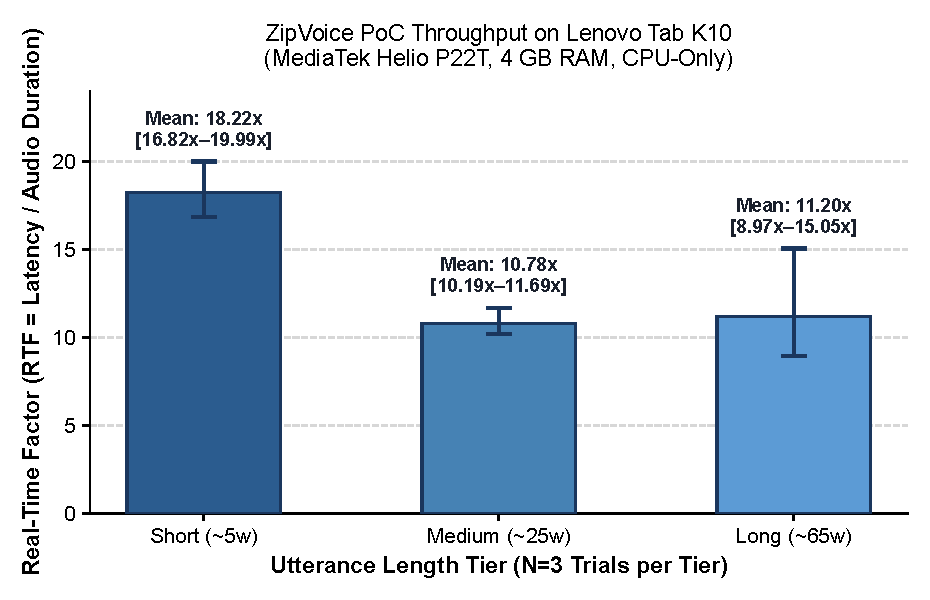
\includegraphics[width=\linewidth]{Figures/lenovo_rtf.pdf}
    \caption[Mean RTF Across Utterance Tiers on Lenovo Tab K10]{Mean Real-Time Factor (\acrshort{rtf}) across utterance tiers on the Lenovo Tab K10 (error bars indicate observed minimum and maximum trial ranges across the three runs, not confidence intervals).}
    \label{fig:lenovo_rtf}
\end{minipage}\hfill
\begin{minipage}{0.48\textwidth}
    \centering
    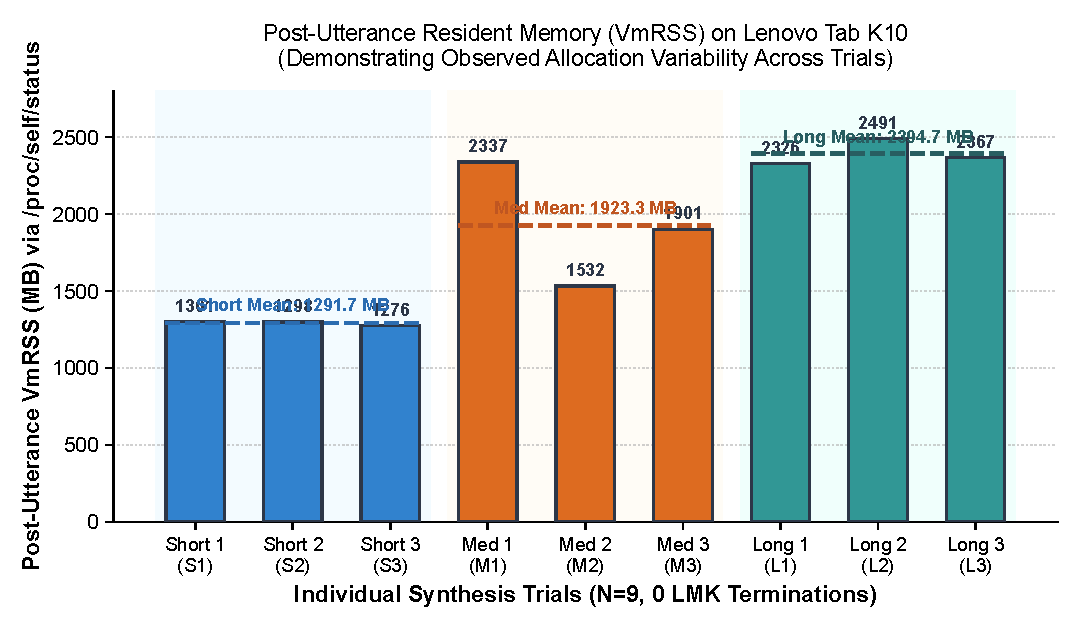
\includegraphics[width=\linewidth]{Figures/lenovo_vmrss.pdf}
    \caption[Post-Utterance Resident Memory on Lenovo Tab K10]{Post-utterance resident memory (\texttt{VmRSS}) across all nine individual trials on the Lenovo Tab K10, showing observed allocation variability across executions.}
    \label{fig:lenovo_vmrss}
\end{minipage}
\end{figure}

\subsection{Analysis of PoC Benchmarks and Inferences for IndicF5 and Google LiteRT}
The empirical benchmarks collected from the ZipVoice PoC across physical hardware tiers yielded four foundational inferences that governed our production system architecture:
\begin{enumerate}
    \item \textbf{Inference 1: Observed Memory Variability and the Rationale for Static Arenas}:
    On the Lenovo Tab K10, all nine experimental trials completed successfully without process termination by the Android low-memory killer. Measured post-utterance resident memory ranged from 1,276\,MB up to 2,491\,MB. These physical readings directly refute the prior hypothesis that exceeding 1,500\,MB resident memory results in an inevitable application termination. 
    
    However, the observations reveal substantial memory variability across trials, including differences within the same length category (for instance, 1,532\,MB versus 2,337\,MB in the medium tier). While the exact sources of this variance require finer-grained profiling (hypothesized causes include sequence-dependent intermediate tensor buffers, retained runtime cache allocations, or native heap allocator behavior), sustained resident memory exceeding 2\,GB increases process vulnerability under multi-tasking conditions. Consequently, static INT8 quantization and pre-allocated memory arenas remain vital engineering priorities for the Indic engine to enforce deterministic memory confinement.
    
    \item \textbf{Inference 2: Characterizing Short-Utterance Latency and Throughput Scaling}:
    Across all evaluated platforms, short utterances exhibited elevated Real-Time Factors (ranging from $3.8\times$ on flagship silicon to a mean of $18.22\times$ on the Tab K10). As sequence duration increased to medium and long tiers, mean RTF stabilized to $10.78\times$ and $11.20\times$ on the K10. While unamortized per-utterance setup costs contribute to elevated short-phrase RTF, establishing an exact latency breakdown across tokenization, session configuration, numerical sampling, and vocoding requires dedicated stage-level instrumentation rather than assuming an invariant cold-start penalty.
    
    \item \textbf{Inference 3: Inadequacy of Off-the-Shelf Mobile Models for Indian Education}:
    Although ZipVoice validated that flow matching can execute on mobile CPUs, its tokenizer and acoustic architecture are fundamentally incapable of processing Dravidian and Indo-Aryan akshara syllabaries, consonant conjuncts, or regional state board textbooks. This confirmed that existing off-the-shelf mobile models cannot simply be repurposed for Indian public schools; rather, a dedicated Indic foundation model (IndicF5) with native character representations across official Indian languages was essential.
    
    \item \textbf{Inference 4: CPU Latency Bounds and the Strategy for Runtime Optimization}:
    On the budget ARM Cortex-A53 cores of the Helio P22T, pure CPU execution demonstrated operational stability but ran substantially slower than real time (RTFs between $8.97\times$ and $19.99\times$). Because the Helio P22T lacks an on-chip Neural Processing Unit, accelerating this budget platform requires CPU-side algorithmic optimizations, specifically sampling step distillation (such as 2-step FlashSpeech consistency models) and runtime buffer reuse. Concurrently, for compatible devices equipped with dedicated silicon, offloading via Google LiteRT delegates (Qualcomm QNN HTP and MediaTek NeuroPilot) forms our hardware acceleration roadmap in \cref{Chapter5}.
\end{enumerate}

\section{Iteration 4: Transition to IndicF5: Multilingual Adaptation and Desktop Verification}
\subsection{Objective: Realizing the PoC Inferences for Indian Languages}
Directly guided by the empirical findings and linguistic limitations discovered during the ZipVoice proof of concept, Iteration~4 transitioned development to our primary production engine: AI4Bharat's IndicF5. The objective was to verify zero-shot vocal cloning across Dravidian and Indo-Aryan languages before undertaking integer quantization and mobile compilation.

\subsection{Model Setup and Adaptation}
We adapted AI4Bharat's IndicF5 repository under \texttt{scratch/indicf5\_repo/}. Developed in PyTorch using safetensors serialization, the base model (\texttt{model.safetensors}) occupied 1.35\,GB in memory. We engineered the standalone command-line verification script \texttt{clone.py} (and \texttt{test\_indicf5\_clone.py}) implementing the continuous flow-matching pipeline with the 22-layer DiT backbone and 24\,kHz Vocos vocoder.

\subsection{Validation Across Indian Languages}
We validated synthesis across four major Indian languages:
\begin{itemize}
    \item \textbf{Tamil}: Synthesizing conversational phrases (e.g., {\tamilfont வணக்கம், நீங்கள் எப்படி இருக்கிறீர்கள்?});
    \item \textbf{Telugu}: Synthesizing conversational phrases (e.g., {\telugufont నమస్కారం, మీరు ఎలా ఉన్నారు?});
    \item \textbf{Kannada}: Testing Kannada phonetic prompts (e.g., \textit{``Namaskara, neevu hegiddira?''}); and
    \item \textbf{Hindi}: Testing Devanagari prompts (e.g., {\indicfont नमस्ते, आप कैसे हैं?}).
\end{itemize}
The model produced intelligible pronunciation without external G2P dictionaries, validating the unified character tokenization approach.

\section{Iteration 5: Syllabic Duration Calibration (Resolving Audio Truncation and Trailing Silence)}
\subsection{The Duration Mismatch Issue}
During early testing with IndicF5, synthesized audio clips suffered from a noticeable duration mismatch:
\begin{quote}
\textit{When synthesizing an Indic sentence, the model articulated target speech with natural prosody during the initial 4 to 5 seconds. However, the generated audio file extended for an additional 6 to 8 seconds, during which the model generated trailing silence, audible breathing, whispered murmurs, repeated syllables, or background noise.}
\end{quote}

\subsection{Root Cause Investigation}
Investigation revealed that the duration allocator utilized an uncalibrated linear heuristic ($T_{\text{gen}} = \text{len}(\mathbf{w}_{\text{tgt}}) \times 15.0$ frames). Because written Indic text contains numerous combining diacritics (\textit{matras}, \textit{viramas}), character string length is inflated relative to spoken syllable counts. Allocating 15 mel frames per Unicode character resulted in a 12.8-second mel canvas for an utterance that naturally completes in 5.2 seconds. 

Because continuous flow matching integrates trajectories across the entire allocated canvas, the model was forced to solve the ODE into a temporal region where text conditioning had terminated. The self-attention layers consequently synthesized low-probability acoustic artifacts (breathing, murmurs, and repeated phonemes).

\subsection{Resolution: Calibrated 6.5 Mel Frames per Character}
As derived in \cref{sec:duration_modeling}, we re-calibrated the temporal density constant to:
\begin{equation}
    k_{\text{mel}} = 6.5 \quad \text{mel frames per character code point}
\end{equation}
With an STFT hop length of $H = 256$ samples at sampling frequency $f_s = 24{,}000$\,Hz, each individual mel frame spans exactly $\Delta t_{\text{frame}} = 256 / 24{,}000 \approx 10.667$\,ms. An allocation of $k_{\text{mel}} = 6.5$ mel frames per Unicode code point corresponds to:
\begin{equation}
    \Delta t_{\text{char}} = 6.5 \times 10.667\,\text{ms} \approx 69.33\,\text{ms per character code point}
\end{equation}
In Indic scripts (such as Tamil, Telugu, and Devanagari), orthographic syllables (\textit{aksharas}) typically comprise approximately 1.6 to 2.2 Unicode code points due to base consonants, vowel signs (\textit{matras}), and viramas. Consequently, an allocation of 6.5 frames per code point yields an effective spoken syllable duration of $\approx 111\text{--}153$\,ms, closely matching natural Indian speech cadences. Post-utterance padding was constrained to an explicit 0.30-second acoustic buffer ($\tau_{\text{pad}} = 28$ frames). This adjustment eliminated trailing artifacts and yielded clean sentence endings across Tamil, Telugu, and Hindi while maintaining linguistic intelligibility.

\section{Iteration 6: Sequence Alignment and Reference Audio Duration Constraints}
\subsection{The Long-Reference Degradation Issue}
In subsequent testing, we observed that when users supplied long reference audio clips (such as a 10.8-second recording, \texttt{sudhanva\_voic\_clone.wav}), the synthesized output degraded into unintelligible static, even when the prompt text was brief.

\subsection{Root Cause Investigation}
We traced this issue to the spatial alignment design of the F5-TTS architecture:
\begin{enumerate}
    \item In F5-TTS, text tokens for the concatenated sequence $[\mathbf{w}_{\text{ref}} \oplus \mathbf{w}_{\text{tgt}}]$ are mapped by ConvNeXt-V2 text blocks into representation vectors that are concatenated along the channel dimension with the noisy acoustic canvas and acoustic prompt.
    \item When a 10.8-second reference audio clip is ingested, $T_{\text{ref}} = 1016$ mel frames. The reference audio occupies the initial 1016 frames, but the text tokens in the fused channel terminate at a much shorter sequence index (corresponding to the character count of the short prompt).
    \item Consequently, target audio synthesis in the temporal region ($t \in [1016, 1500]$ frames) occurred where text representation features were completely zero-padded. Under bidirectional self-attention with Rotary Position Embeddings (RoPE) stretched across such large temporal offsets, the model suffered from attention dispersion and diluted contextual grounding, synthesizing unconditioned noise.
\end{enumerate}

\subsection{Resolution: Reference Duration Recommendation}
Based on preliminary synthesis experiments, we recommend reference audio clips between 3.5 and 5.0 seconds for the evaluated IndicF5 configuration ($T_{\text{ref}} \in [328, 468]$ frames). We recorded and verified clean, phonetically balanced 3.8-second reference clips (\texttt{sudhanva\_short\_ref.wav} and \texttt{tamil\_classic\_pangram.mp3} in \texttt{samples/}). When paired with verbatim reference transcripts, spatial text-mel alignment was maintained, restoring clear phonetic articulation.

\section{Iteration 7: In-Memory Warm Model Batch Synthesis and Dataset Curation}
\subsection{Motivation and Batch Engine}
Iterative model validation required evaluating multiple sentences across diverse speakers, languages, and duration tiers. Loading the 1.35\,GB PyTorch model weights from disk on every invocation incurred a 12-second cold-start penalty per sentence.

\subsection{System Architecture}
We engineered the dedicated batch synthesis engine \texttt{batch.py} within the backend architecture:
\begin{itemize}
    \item \textbf{In-Memory Model Caching}: The 1.35\,GB model weights, vocabularies, and Vocos vocoder are loaded into RAM once during initialization. Subsequent synthesis requests reuse the warm pipeline, eliminating cold-load latency.
    \item \textbf{Auto-Incrementing Batch Storage}: Each execution automatically creates the next incremental output directory (\texttt{generated/batches/batch-1/}, \texttt{batch-2/}, etc.).
    \item \textbf{Multi-Processing Concurrency}: Implemented an optional multi-worker process pool (\texttt{--parallel --workers N}) utilizing inter-process queues for parallel benchmark throughput.
\end{itemize}

\subsection{The Multilingual Dataset (\texttt{prompts.json})}
To standardize evaluation, we authored the curated dataset \texttt{prompts.json}, comprising 120 authentic conversational phrases across Tamil, Telugu, and Hindi. To evaluate latency and duration scaling systematically, the dataset is stratified into four standardized tiers:
\begin{enumerate}
    \item \textbf{Short Tier} (10 phrases/language, 4--7 words): Everyday conversational greetings and inquiries.
    \item \textbf{Medium Tier} (10 phrases/language, 12--18 words): Moderate-length social dialogues.
    \item \textbf{Midlong Tier} (10 phrases/language, 20--25 words): Compound sentences describing activities and settings.
    \item \textbf{Long Tier} (10 phrases/language, 28--35 words): Complex narrative sentences with multiple dependent clauses.
\end{enumerate}

\section{Iteration 8: Unified Voice Studio Suite and Dynamic Catalog Management}
\subsection{System Architecture}
To establish a modular codebase, the backend was refactored into the Python package \texttt{src/voice\_studio/}, organized as follows:
\begin{itemize}
    \item \texttt{config.py}: Centralized path resolutions, hardware constants, and UTF-8 stream configurations.
    \item \texttt{audio/io.py}: Format decoding, FFmpeg transcoding, and RMS normalization.
    \item \texttt{catalog/manager.py}: Voice catalog CRUD operations, automatic metadata extraction, and audio validation.
    \item \texttt{dataset/prompts.py}: Tier-based phrase parsing and range selection.
    \item \texttt{engines/}: Unified engine interfaces for IndicF5, ZipVoice, and batch runner execution.
    \item \texttt{cli/}: Unified entry point via \texttt{main.py}, supporting an interactive Terminal User Interface (TUI) and direct subcommands (\texttt{list}, \texttt{info}, \texttt{add}, \texttt{prompts}, \texttt{clone}, \texttt{batch}).
\end{itemize}

\subsection{Dynamic Catalog Management (\texttt{samples/voices.json})}
The catalog tracks registered speaker reference clips, storing voice keys, spoken transcripts, descriptions, audio durations, and creation timestamps. In an educational setting, this catalog enables teachers across different academic subjects (such as Mathematics, Science, and Regional Literature) to register distinct instructor profiles. When a teacher registers a new voice via \texttt{python main.py add}, the system validates audio integrity, measures duration, normalizes RMS energy, and stores the file into \texttt{samples/added/}. This structure allows students, particularly visually impaired learners who rely entirely on audio lessons, to select and listen to content voiced by their specific subject teacher.

\section[Iteration 9: Graph Optimization and INT8 Quantization]{Iteration 9: Graph Optimization, FP32 Export, and Static/Dynamic INT8 Quantization}
\subsection{Objective: Decoupling from the PyTorch Runtime}
Deploying IndicF5 onto Android devices requires decoupling the model from the heavy Python runtime, Librosa, and PyTorch (which exceed 2.5\,GB on disk). Iteration~9 developed the complete graph optimization and integer quantization export pipeline under \texttt{models/indicf5/}.

\subsection{Exported Model Artifacts and Sequence Dimension Formulation}
We exported and verified the core model artifacts comprising four ONNX graphs, the baseline PyTorch checkpoint, and the standalone tokenizer vocabulary:
\begin{enumerate}
    \item \textbf{\texttt{model.safetensors}}: Baseline PyTorch weights (1.35\,GB, 335M parameters).
    \item \textbf{\texttt{indicf5\_dit\_fp32\_static.onnx}}: Static-shape unquantized FP32 graph (1.36\,GB, fixed at 128 mel frames for baseline numerical equivalence testing).
    \item \textbf{\texttt{indicf5\_dit\_dynamic\_fp32.onnx}}: Dynamic sequence dimension FP32 graph (1.36\,GB, supporting variable audio lengths for desktop evaluation).
    \item \textbf{\texttt{indicf5\_dit\_int8\_static.onnx}}: Static INT8 post-training quantized DiT graph (~349\,MB, 74\% size reduction). Here, ``static'' denotes both static calibration of activation quantization parameters and a fixed 128-frame tensor dimension ($T=128$) engineered specifically as an optimization and export prototype for deterministic memory arena benchmarking.
    \item \textbf{\texttt{indicf5\_vocos\_int8.onnx}}: INT8 quantized Vocos neural vocoder (~22\,MB, down from 54\,MB in FP32).
    \item \textbf{\texttt{vocab.txt}}: Standalone multilingual character tokenization mapping (11.3\,KB, 187 tokens).
\end{enumerate}

To ensure academic and technical precision, we must explicitly clarify the functional distinction between fixed-shape and variable-length artifacts. In speech synthesis at 24\,kHz ($H=256$), a typical 3.5-second reference audio clip alone corresponds to approximately 328 mel frames ($T_{\text{ref}} \approx 328$). Consequently, the fixed 128-frame static INT8 model cannot ingest complete reference voice prompts or arbitrary educational passages. Instead, this graph represents a successfully exported \textbf{optimization prototype} designed to confirm that 8-bit integer quantization preserves numerical stability without divergence, and to benchmark physical memory confinement in fixed memory arenas. 

Verified end-to-end variable-length synthesis is currently achieved on desktop environments utilizing the unquantized dynamic-axis FP32 graph (\texttt{indicf5\_dit\_dynamic\_fp32.onnx}). Naive temporal chunking of mel frames cannot be applied to F5-TTS because its non-autoregressive DiT relies on bidirectional self-attention and Rotary Position Embeddings spanning the concatenated prompt-and-target sequence; chunking into isolated 128-frame blocks would sever acoustic conditioning and degrade prosodic continuity. Therefore, exporting a dynamic-axis INT8 graph and integrating dynamic tensor management within the native C++ runtime is designated as our primary post-mid-semester deployment milestone.

\section{Iteration 10: Custom Native C++ Engine and Dart FFI Shared Library}
\subsection{Motivation}
Because \texttt{sherpa-onnx} lacks built-in C++ loaders for Diffusion Transformers and F5-TTS, we engineered a dedicated native shared library (\texttt{libindicf5\_engine.so}) linking directly to the ONNX Runtime Mobile C++ API.

\subsection{C++ Engine Architecture (\texttt{indicf5\_engine.cpp})}
The native engine implements:
\begin{itemize}
    \item Direct session initialization using the ONNX Runtime C++ API for the fixed-shape INT8 DiT prototype and the quantized Vocos vocoder, validating native model loading and tensor lifecycle management.
    \item Pre-allocated static tensor arenas (280\,MB), eliminating dynamic heap allocations across the 8 Euler ODE integration steps for fixed-dimension tensors.
    \item Native implementation of the Classifier-Free Guidance Euler update step:
    \begin{equation}
        x_{t+\Delta t}[k] = x_t[k] + \Delta t \cdot \left( (1 + \gamma) v_{\text{cond}}[k] - \gamma v_{\text{uncond}}[k] \right)
    \end{equation}
    accelerated via multi-threaded ARM NEON execution kernels.
    \item A C ABI interface (\texttt{indicf5\_c\_api.h}) exposing core lifecycle and synthesis routines (\texttt{indicf5\_create}, \texttt{indicf5\_synthesize}, \texttt{indicf5\_destroy}).
    \item A Dart FFI bridge service (\texttt{indicf5\_service.dart}) enabling the Flutter application to invoke native C++ inference in background Dart Isolates without bridging overhead.
\end{itemize}
Thus, while native loading and memory arena pre-allocation are functionally validated with the static INT8 prototype, full end-to-end on-device execution of arbitrary-length classroom utterances remains scheduled for post-mid-semester validation following dynamic-axis INT8 model compilation.

\begin{figure}[htbp]
\centering
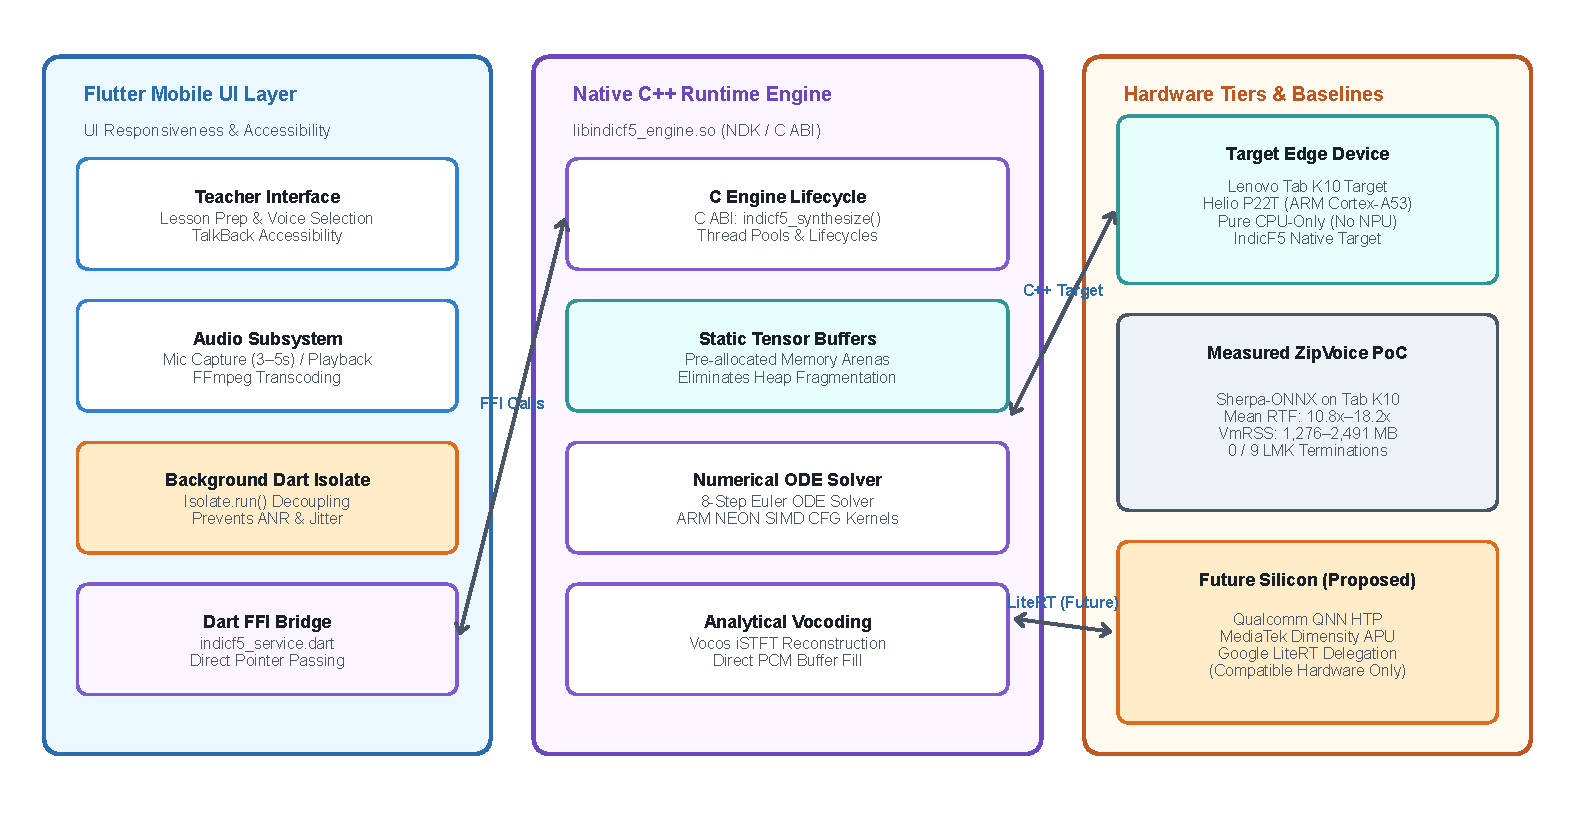
\includegraphics[width=0.92\textwidth]{Figures/runtime_architecture.pdf}
\caption[Native IndicF5 Runtime and Edge Deployment Architecture]{Native runtime and deployment architecture for on-device Indic voice synthesis, illustrating the interaction between the Flutter UI, Dart FFI bridge, native C++ engine, and the ONNX Runtime session with static memory arenas.}
\label{fig:runtime_architecture}
\end{figure}

\section{Hardware Memory Budget Analysis on \texorpdfstring{4\,GB}{4 GB} RAM Platforms}
To evaluate the memory feasibility of deploying the proposed quantized IndicF5 pipeline within a 4\,GB physical RAM envelope, Table~\ref{tab:ram_budget_comparison} details an analytical component-level memory budget. 

It is essential to emphasize that the proposed quantized architecture has an analytical component budget of approximately 801\,MB; its actual process memory footprint remains subject to validation on target Android hardware. This 801\,MB figure represents a calculated theoretical sum of model weights, static working buffers, and runtime estimates, rather than a physically measured process Resident Set Size (\acrshort{rss}) or an experimentally proven upper bound. In physical edge execution, actual Android process RSS can differ substantially due to runtime dynamic heap allocations, memory-mapped model weights, intermediate tensor activations, shared libraries, Flutter engine graphic surfaces, and underlying OS memory allocator behavior.

Importantly, the empirical memory readings observed during the ZipVoice PoC on the Lenovo Tab K10 (where post-utterance resident memory reached up to 2,491\,MB without LowMemoryKiller termination) illustrate that Android processes can survive high physical memory occupancy depending on system-wide memory pressure; however, because ZipVoice and IndicF5 represent fundamentally distinct model architectures and execution runtimes, their physical memory footprints cannot be directly equated.

\begin{table}[htbp]
\centering
\caption[Analytical Memory Budget for Proposed Quantized IndicF5 Deployment]{Analytical Memory Budget for the Proposed Quantized IndicF5 Deployment on 4\,GB Android Hardware}
\label{tab:ram_budget_comparison}
\resizebox{\textwidth}{!}{%
\begin{tabular}{lcc}
\toprule
\textbf{Memory Subsystem Component} & \textbf{Unquantized Baseline (FP32)} & \textbf{Quantized System (Analytical Estimate)} \\
\midrule
Diffusion Transformer (DiT) Weights & 1,350\,MB & 349\,MB (Static INT8) \\
Vocos Neural Vocoder Weights & 54\,MB & 22\,MB (INT8) \\
Inference Working Arenas & 850\,MB (Heap, up to 1,200\,MB) & 280\,MB (Pre-allocated Static) \\
Flutter Runtime, Dart VM \& UI Buffers & 150\,MB & 150\,MB \\
\midrule
\textbf{Analytical Component Total} & \textbf{2,404\,MB} & \textbf{801\,MB} \\
\midrule
\multicolumn{3}{l}{\textit{Engineering Planning Context:}} \\
Engineering Planning Reference Target & $\approx 1,500$\,MB & $\approx 1,500$\,MB (Nominal Edge Budget) \\
Analytical Design Alignment & Exceeds Reference & Within Planning Target ($-699$\,MB Target Margin) \\
\bottomrule
\end{tabular}%
}
\vspace{0.6ex}
\begin{minipage}{\textwidth}
\footnotesize
\textit{Note}: The 801\,MB total is an analytical component-level estimate, not a measured Android process RSS or an operating-system-enforced threshold. Actual process memory footprint on physical edge hardware remains subject to empirical validation.
\end{minipage}
\end{table}

By establishing an analytical component budget of approximately 801\,MB, the quantized architecture provides a concrete design target for edge deployment on 4\,GB platforms, aligning within our nominal 1,500\,MB engineering planning envelope while physical memory validation is undertaken in subsequent on-device trials.

\section{Evaluation Limitations and Future Validation Plan}
\label{sec:eval_limitations}
While the experimental results and engineering iterations demonstrate the architectural feasibility of on-device Indic voice synthesis, several rigorous empirical evaluations remain planned for post-mid-semester investigation:
\begin{enumerate}
    \item \textbf{Objective Voice Quality and Naturalness}: Perceptual evaluation of synthesized speech quality (via Mean Opinion Score listening tests, Word Error Rate, and Character Error Rate using pretrained Whisper/Wav2Vec2 models) across varying sampling step counts ($N \in \{2, 4, 8, 16\}$).
    \item \textbf{Speaker Similarity and Verification}: Quantitative evaluation of zero-shot speaker cloning fidelity using cosine similarity of deep speaker embeddings (ECAPA-TDNN and WavLM) between reference teacher recordings and synthesized audio.
    \item \textbf{Acoustic Quality Retention under INT8 Quantization}: Comprehensive comparative measurement of audio degradation, spectral distortion, and objective speech intelligibility between FP32 PyTorch baseline checkpoints and INT8 quantized ONNX graphs.
    \item \textbf{Quantized IndicF5 On-Device Profiling}: While the ZipVoice proof of concept was thoroughly benchmarked on physical hardware (including the Lenovo Tab K10), on-device latency and resident memory profiling for the custom C++ IndicF5 runtime on target Android hardware will be completed following deployment stabilization.
    \item \textbf{Acoustic Robustness to Classroom Recording Conditions}: Controlled evaluation of reference voice adaptation under realistic classroom ambient noise (reverberation, background murmur, and microphone clipping) common in public school settings.
\end{enumerate}